\documentclass[tikz,border=2pt]{standalone}
\usepackage{amsmath,amssymb}
\usepackage{tikz}
\usetikzlibrary{matrix,arrows.meta}

\begin{document}
% Entering variable rule (maximisation tableau): pick the nonbasic column with the most
% negative objective-row coefficient; here -3 for x_s, so x_s enters the basis.
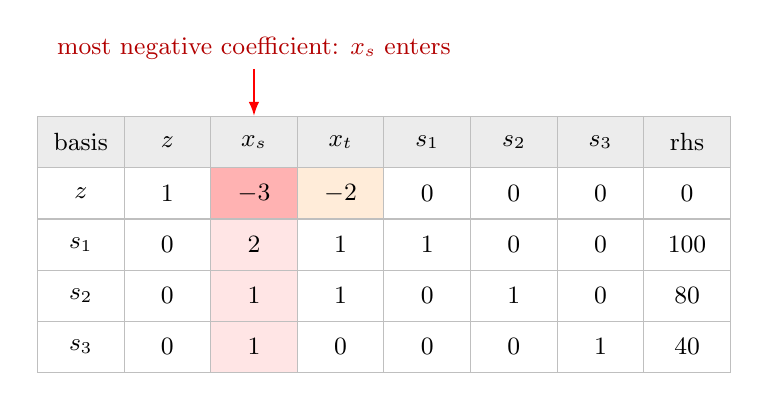
\begin{tikzpicture}[every node/.style={font=\small}, >={Latex[length=1.8mm]}]
	\matrix (T) [matrix of math nodes, nodes={minimum width=1.1cm, minimum height=6.5mm, anchor=center, draw=gray!50}, column sep=-\pgflinewidth, row sep=-\pgflinewidth] at (0,0) {
		|[fill=gray!15]| \text{basis} & |[fill=gray!15]| z & |[fill=gray!15]| x_s & |[fill=gray!15]| x_t & |[fill=gray!15]| s_1 & |[fill=gray!15]| s_2 & |[fill=gray!15]| s_3 & |[fill=gray!15]| \text{rhs} \\
		z & 1 & |[fill=red!30]| -3 & |[fill=orange!15]| -2 & 0 & 0 & 0 & 0 \\
		s_1 & 0 & |[fill=red!10]| 2 & 1 & 1 & 0 & 0 & 100 \\
		s_2 & 0 & |[fill=red!10]| 1 & 1 & 0 & 1 & 0 & 80 \\
		s_3 & 0 & |[fill=red!10]| 1 & 0 & 0 & 0 & 1 & 40 \\
	};
	\draw[->, red, thick] (T-1-3.north) ++(0,0.6) -- (T-1-3.north);
	\node[red!70!black, anchor=south] at ([yshift=0.6cm]T-1-3.north) {most negative coefficient: $x_s$ enters};
	\end{tikzpicture}
\end{document}
